\begin{table*}[t]
\caption{Main results under the 2\,s end-to-end budget (two repeats per task). Correct: outcome equals the reference. Wrong: answered but different from the reference; for a certified answer this is a soundness failure (none occurred). PAR-2: ancestor-equal mean, 4\,s for an unanswered or wrong run; best certified method per suite in bold. PAR-10w charges a wrong answer 20\,s instead (it differs from PAR-2 only for uncertified methods). $^\ast$added in stage~2; $^\ddagger$SAT encoding solved by CaDiCaL, added in stage~3; $^\dagger$post hoc arm on Hard and HPRD. Priors predict labels without search, leave one ancestor out, counted per run.}
\label{tab:main}
\centering\small\setlength{\tabcolsep}{4.5pt}
\begin{tabular}{l rrr rrr rrr}
\toprule
 & \multicolumn{3}{c}{IdCon-Hard (1,008 runs)} & \multicolumn{3}{c}{IdCon-HPRD (400 runs)} & \multicolumn{3}{c}{IdCon-HPRD-X (384 runs)}\\
\cmidrule(lr){2-4}\cmidrule(lr){5-7}\cmidrule(lr){8-10}
Method & Correct & Wrong & PAR-2 & Correct & Wrong & PAR-2 & Correct & Wrong & PAR-2\\
\midrule
LAD & 725 & 0 & \textbf{1,635} & 389 & 0 & 1,036 & 199 & 0 & 2,513\\
Glasgow & 562 & 0 & 2,113 & 0 & 0 & 4,000 & 1 & 0 & 3,995\\
Glasgow-staged$^\dagger$ & 651 & 0 & 1,740 & 304 & 0 & 1,361 & 265 & 0 & 1,734\\
CP-SAT & 321 & 0 & 2,998 & 384 & 0 & 455 & 360 & 0 & 830\\
Trad-CP & 214 & 0 & 3,347 & 279 & 0 & 1,858 & 191 & 0 & 2,603\\
Enum-Glasgow$^\ast$ & 88 & 0 & 3,688 & 235 & 0 & 2,638 & 65 & 0 & 3,568\\
Enum-VF2$^\ast$ & 14 & 0 & 3,951 & 127 & 0 & 2,937 & 74 & 0 & 3,354\\
ASP-cautious$^\ast$ & 15 & 0 & 3,968 & 400 & 0 & 748 & 365 & 0 & 1,230\\
SAT$^\ddagger$ & 240 & 0 & 3,378 & 400 & 0 & \textbf{374} & 384 & 0 & \textbf{380}\\
\midrule
First-match (PAR-2 / PAR-10w) & 626 & 315 & 1,901 / 6,901 & 230 & 170 & 2,027 / 8,827 & 224 & 160 & 2,242 / 8,909\\
Metadata prior & 736 & 272 & -- & 366 & 34 & -- & 328 & 56 & --\\
Learned prior & 838 & 170 & -- & 362 & 38 & -- & 332 & 52 & --\\
\bottomrule
\end{tabular}
\end{table*}


\subsection{Embeddings are rarely unique; first-match is wrong where they disagree}
\label{sec:firstmatch}
What carries over to other workloads is how often embeddings are not unique, which does not depend on our observation rule. Counting embeddings with Glasgow (30~s per query), \hprdCountFullMulti{} of the \hprdCountFullQueries{} IdCon-HPRD queries have more than one embedding when every query vertex must match its own label, and \hprdAutoOrbitMulti{} still do after dividing by the number of label-preserving automorphisms of the query, i.e., counting genuinely different placements (\hprdCountFullThousand{} queries have at least 1,000 embeddings; no count hit the time limit); on IdCon-HPRD-X the figures are \hprdxCountFullMulti{} and \hprdxAutoOrbitMulti{} of \hprdxCountFullQueries{}. With the checked roles freed, \hprdCountSpaceMulti{} and \hprdxCountSpaceMulti{} of the identity spaces have more than one identity.

A first match can be wrong only on an \Unk{} task: if the reference is \Sat{} or \Vio{} every identity has that state, and if it is \Emp{} there is nothing to report. Every wrong first-match run in IdCon is indeed on an \Unk{} task (\hardFirstWrongOnUnknown{} of \hardFirstWrong{} on IdCon-Hard, \hprdFirstWrongOnUnknown{} of \hprdFirstWrong{} on IdCon-HPRD, \hprdxFirstWrongOnUnknown{} of \hprdxFirstWrong{} on IdCon-HPRD-X; Table~\ref{tab:main}). Its error rate on a suite is therefore the share of tasks whose embeddings disagree, a property of the workload rather than a finding: \hardFirstWrongAnsweredPct\% of answered IdCon-Hard runs, set by the generator's decoy rates, and \hprdFirstWrongPct\% of IdCon-HPRD runs, set by the observation rule (\hprdFirstWrongSpecTrue{} of the \hprdFirstWrong{} wrong runs are \textsf{spec\_true} tasks).

\subsection{Exact methods are sound, and none dominates}
\label{sec:exact}
No exact method returned a certified outcome that contradicts a reference on any suite, and all \witnessTotalRtwo{} positive witnesses returned by methods on the five scored suites replay against the original constraints. On IdCon-Hard, \hardBest{} has the lowest PAR-2 (\hardBestPar~ms; runner-up \hardSecond{}, \hardSecondPar~ms). On IdCon-HPRD and IdCon-HPRD-X, \hprdBest{} and \hprdxBest{} have (\hprdBestPar{} and \hprdxBestPar~ms; runners-up \hprdSecond{} and \hprdxSecond{}, \hprdSecondPar{} and \hprdxSecondPar~ms), and \hprdMost{} and \hprdxMost{} answer the most runs (\hprdMostCorrect{} of \hprdASPcautiousAssessed{} and \hprdxMostCorrect{} of \hprdxASPcautiousAssessed{}). The SAT baseline thus leads where label domains are narrow, yet answers only \hardSATCorrect{} of \hardSATAssessed{} IdCon-Hard runs, where its encoding grows with the number of candidates per role. Inside the suites the best method changes with size, anchoring and query size (Appendix Figure~\ref{fig:strata} and Tables~\ref{tab:strata-hard}--\ref{tab:strata-hprdx}); with the share of bootstrap resamples in which it stays best in brackets, and n.s.\ where it is not distinguishable from the runner-up, \strataSentence{}. With 12 ancestors per IdCon-Hard stratum these comparisons are coarse. At 2\,s the best single method leaves \hardBestUnsolvedPct\% of IdCon-Hard runs unsolved; a VBS over the methods registered in stages 1 and 2 (Glasgow-staged excluded as a post hoc arm) leaves \hardVBSUnsolved{} runs (\hardVBSUnsolvedPct\%), and one over every sound method including Glasgow-staged and SAT leaves \hardVBSAllUnsolved{} (\hardVBSAllUnsolvedPct\%). These figures describe the benchmarked methods at 2\,s, not a limit of exact methods: two unpublished solvers of the authors, run in stage~1 and not part of the benchmark, answer \legEgCorrect{} and \legSvCorrect{} of the 1,008 IdCon-Hard runs at 2\,s, and with them the VBS leaves \legVBSBoth{} (Appendix Table~\ref{tab:legacy}).

\begin{table}[t]
\caption{Stage-3 suites (repeat~0, one run per task and budget on IdCon-Hard-X; two repeats at 2\,s on IdCon-Cite). Correct runs within 2, 10 and 60\,s (a run unanswered at a budget is rerun at the next for the methods listed in the design record; -- not rerun). VBS: tasks that no sound method answers within the budget. No certified answer contradicts a reference.}
\label{tab:newsuites}
\centering\footnotesize
\setlength{\tabcolsep}{2.6pt}
\begin{tabular}{lrrr rrr}
\toprule
 & \multicolumn{3}{c}{IdCon-Hard-X (68 tasks)} & \multicolumn{3}{c}{IdCon-Cite (192 tasks)}\\
\cmidrule(lr){2-4}\cmidrule(lr){5-7}
Method & 2\,s & 10\,s & 60\,s & 2\,s$^{2}$ & PAR-2 & 10\,s\\
\midrule
LAD & 1 & 30 & 64 & 192 & 2,086 & 191\\
Glasgow & 1 & 29 & -- & 92 & 3,256 & --\\
Glasgow-staged & 15 & 33 & 46 & 126 & 2,904 & 107\\
CP-SAT & 5 & 11 & -- & 124 & 2,911 & 88\\
Trad-CP & -- & -- & -- & 190 & 2,188 & --\\
Enum-Glasgow$^\ast$ & 1 & 4 & -- & 104 & 3,118 & --\\
Enum-VF2$^\ast$ & -- & -- & -- & 77 & 3,300 & --\\
ASP-cautious$^\ast$ & -- & -- & -- & 223 & 1,964 & 192\\
SAT$^\ddagger$ & 2 & 2 & 40 & 265 & 1,598 & 192\\
\midrule
First-match & 1 & 35 & -- & 114 & 2,837 & --\\
\midrule
VBS unsolved & 49 & 23 & 3 & 110 & -- & 0\\
\bottomrule
\end{tabular}
\end{table}


\subsection{Larger hosts and real labels}
\label{sec:newsuites}
The stage-3 suites change the picture where IdCon-Hard is near saturation (Table~\ref{tab:newsuites}). On IdCon-Hard-X, where one LAD2025 query alone takes about 3\,s on a 16,384-entity host, the methods jointly leave \hardxVBSUnsolvedTwo{} of \hardxComplete{} assessed tasks unanswered at 2\,s, \hardxVBSUnsolvedTen{} at 10\,s and \hardxVBSUnsolvedSixty{} at 60\,s; the best single method answers \hardxBestSingleTenN{} within 10\,s (\hardxBestSingleTen{}) and \hardxBestSingleSixtyN{} within 60\,s (\hardxBestSingleSixty{}). Glasgow-staged answers most at 2\,s, LAD after its slow first query. On IdCon-Cite, whose few labels leave wide domains on real citation graphs, the fastest sound method is \citeBest{} (PAR-2 \citeBestPar~ms), the certain-answer formulations (ASP-cautious, SAT) are competitive with the two-query adapters, and the methods jointly leave \citeVBSUnsolvedRuns{} of the 2\,s runs unanswered and \citeVBSUnsolvedTen{} tasks at 10\,s. No certified answer contradicts a reference on either suite.

\begin{figure*}[t]
\centering
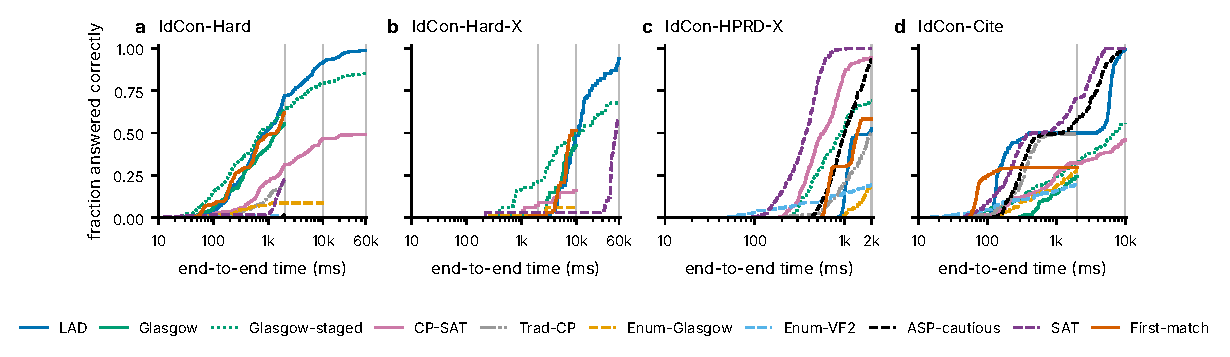
\includegraphics[width=\textwidth]{figures/fig2_results.pdf}
\caption{Fraction of assessed tasks answered correctly within a given end-to-end time (repeat~0). Runs unanswered at 2\,s continue with the 10\,s rerun and, for the methods rerun at 60\,s, with the 60\,s rerun (grey lines: 2, 10 and 60\,s). (a) IdCon-Hard, (b) IdCon-Hard-X, (c) IdCon-HPRD-X, (d) IdCon-Cite. Dashed: methods added in stages 2 and 3. Times after the first budget on IdCon-Hard come from the stage-3 machine (\calibRatio{} times slower).}
\label{fig:results}
\end{figure*}

\subsection{Budget, overhead and headroom}
\label{sec:budget}
The difficulty of IdCon-Hard is largely a 2\,s difficulty (Figure~\ref{fig:results}a). On repeat~0, LAD answers \hardLadRepTwo{} of 504 tasks at 2\,s, \hardLadRepTen{} at 10\,s and \hardLadRepSixty{} at 60\,s; the VBS over every sound method leaves \hardVBSAllUnsolvedTwo{}, \hardVBSAllUnsolvedTen{} and \hardVBSAllUnsolvedSixty{} tasks unanswered (at 60\,s: \hardVBSSixtyLabels{}). IdCon-Hard therefore separates methods at short budgets and is close to solved with a minute per task; IdCon-Hard-X separates them at 10\,s (Section~\ref{sec:newsuites}). On IdCon-HPRD every method rerun at 10\,s reaches at least \hprdGlasgowTenS{} of \hprdRepZeroN{} tasks, and ASP-cautious and SAT answer \hprdASPcautiousCorrect{} and \hprdSATCorrect{} of its \hprdSATAssessed{} runs at 2\,s; that suite's 2\,s ranking measures per-call start-up cost more than search. The cost is visible directly. On IdCon-HPRD one LAD call on a one-role pattern takes \ovhLadOneRole~ms end to end and one default Glasgow call \ovhGlasgowOneRole~ms. On 48 stratified IdCon-Hard tasks, the first LAD query takes \ovhHardLadTotal~ms (median), of which \ovhHardLadOutside~ms are spent outside the solver process (building the graph, writing files) and the solver process \ovhHardLadSolver~ms; for Glasgow-staged the figures are \ovhHardGSTotal, \ovhHardGSOutside{} and \ovhHardGSSolver~ms. Results at one budget should be read with the completion curves, and adapter engineering is part of what the 2\,s budget measures.

\subsection{Tools and universal outcomes}
\label{sec:tools}
On IdCon-Hard, where by degree almost every entity is a candidate for every role, enumeration and grounding do not finish: Enum-Glasgow answers \hardEnumGlasgowCorrect{}, Enum-VF2 \hardEnumVFTwoCorrect{} and ASP-cautious \hardASPcautiousCorrect{} of \hardEnumGlasgowAssessed{} runs. Where label domains are narrow (HPRD) the certain-answer formulations are the most complete methods: ASP-cautious and SAT answer \hprdxASPcautiousCorrect{} and \hprdxSATCorrect{} of the \hprdxSATAssessed{} IdCon-HPRD-X runs. \Unk{} needs witnesses only, whereas \Sat{}, \Vio{} and \Emp{} need a completed negative search, and the methods differ most on the latter: on IdCon-Hard, LAD answers \hardLADSatCorrect{} \Sat{} runs and CP-SAT \hardCPSATSatCorrect{}, against \hardLADUnkCorrect{} and \hardCPSATUnkCorrect{} \Unk{} runs (Appendix Table~\ref{tab:labels}).

\subsection{What can be predicted without search}
\label{sec:prior}
On IdCon-Hard the scenario alone predicts \hardPriorScenario{} references, all metadata \hardPriorMeta{}, and the learned prior \hardPriorLearned{} (\hardPriorLearnedPct\%); \priorWrongAllThree{} references defeat all three priors. Two shortcuts explain much of this. First, in \sensDecided{} tasks (\sensDecidedPct\%; \sensDecidedDecoyS{} of them the \textsf{decoy\_s} control) the observation tables exclude two of the three states in a scenario whose construction embedding is admissible, so one existence query decides the label; a method that adds this table check gains these runs. Second, on the HPRD suites the scenario fixes the label for \hprdPriorScenario{} and \hprdxPriorScenario{} tasks, because a misstated label is rarely carried by an admissible embedding. The ranking of the exact methods is robust to both: without \textsf{decoy\_s} and without all \sensDecided{} table-decided tasks, \sensRankSentence{} (post hoc, Appendix Table~\ref{tab:sensitivity}). On IdCon-Hard-X and IdCon-Cite the learned prior reaches \hardxPriorLearned{} and \citePriorLearned{}. A learned predictor has to beat these numbers before its accuracy reflects the graph; for exact methods the shortcuts only mean that part of a suite is easy. Because the released tools compute exact labels from public inputs (IdCon-HPRD-H) or from a public seed (IdCon-Hard-H), the held-out splits guard against tuning, not against a determined user.

\begin{table}[t]
\caption{Independent reference check: an encoding written without any benchmark code, solved by CaDiCaL; witnesses replayed against the raw input; negatives decided on the unpruned encoding with DRAT proofs verified by drat-trim. Settles: tasks \textsc{Unassessed} in the reference that the check decides. Limits: 600\,s per solve and 1,200\,s per proof check (registered) for the first 4 tasks, 120\,s and 300\,s for the rest (Amendment~6); Hard-X single-engine negatives: every IdCon-Hard-X task with a negative state that only one reference engine established, not already sampled (Amendment~7).}
\label{tab:idcheck}
\centering\footnotesize
\setlength{\tabcolsep}{3pt}
\begin{tabular}{lrrrrr}
\toprule
Sample & Tasks & Agree & Disagree & Unresolved & Settles\\
\midrule
Hard, unconfirmed negative & 17 & 10 & 0 & 7 & 0\\
Hard, stratified random & 48 & 44 & 0 & 4 & 0\\
HPRD-X, no ASP answer & 4 & 4 & 0 & 0 & 0\\
Cite, all tasks & 192 & 192 & 0 & 0 & 0\\
Hard-X, one per ancestor & 12 & 10 & 0 & 1 & 1\\
Hard-X, single-engine negative & 19 & 19 & 0 & 0 & 0\\
\midrule
Total & 292 & 279 & 0 & 12 & 1\\
\bottomrule
\end{tabular}
\end{table}


\subsection{Reference quality}
\label{sec:refquality}
Every positive state is a replayed witness. Of the \hardNegRone{} non-trivial IdCon-Hard negatives, \hardNegRoneCorroborated{} are confirmed by a second engine after the stage-2 re-check (\hardNegVoneCorroborated{} of \hardNegVone{} after stage~1); on IdCon-HPRD all \hprdNegRone{} are, and on IdCon-HPRD-X \hprdxNegRoneCorroborated{} of \hprdxNegRone{}. The second engines are themselves benchmarked and share the adapters' code, so we added the independent check of Section~\ref{sec:protocol} (Table~\ref{tab:idcheck}): it decides \idcDecided{} of \idcTasks{} sampled and new-suite tasks, agrees with \idcAgree{} references, contradicts \idcDisagree{} and decides \idcSettles{} that the reference procedure left \textsc{Unassessed} (\idcUnresolved{} unresolved; \idcDrat{} negative states carry verified DRAT proofs), including \idcUnconfAgree{} of the \idcUnconfTasks{} IdCon-Hard tasks whose negatives no second engine had confirmed. The new suites need it most on IdCon-Hard-X, where Glasgow corroborates only \hardxNegCorroborated{} of \hardxNeg{} non-trivial negatives within its 30\,s on the 16,384-entity hosts (IdCon-Cite: \citeNegCorroborated{} of \citeNeg{}); the check agrees on \idcHardxSingleAgree{} of the \idcHardxSingleTasks{} IdCon-Hard-X tasks with such a single-engine negative (\idcHardxSingleUnresolved{} unresolved) and on \idcCiteAgree{} of \idcCiteTasks{} IdCon-Cite tasks. Restricted to fully confirmed references, the ranking of the sound methods \refRankSentence{} (Appendix Table~\ref{tab:refs}).
